\ifx\wholebook\relax\else
\input{../Common.tex}
\input{../macroes.tex}
\begin{document}
\fi

\chapter{Conditional Loops}\label{ch:ConditionalLoops}

Conditions are a powerful tools for expressing complex programs. However, conditions are not enough. Some programs need to combine loops and conditions. Loops and conditions are combined in conditional loops, \ie\ loops that execute a block of expressions while a certain condition holds. This chapter presents the conditional loops offered by \st and go over simple examples. We will use a lot conditional loops to simulate animal behavior  in Chapter~\ref{ch:simulateAni}.

\section{Conditional Loops}
The idea behind conditional loops is that a block (a sequence of expressions) is repeated as long as a certain condition holds. \st defines two messages, \index{whileTrue:}\ct{whileTrue:} and \index{whileFalse:}\ct{whileFalse:}, that allow you to define conditional loops as shown  below. 

\paragraph{An Example.} Let's take a simple example to illustrate their use.  Imagine we want a robot to move  north until its y coordinate is smaller than 100 pixels as shown in Figure~\ref{fig:PointingNorth}.  A solution using a conditional loop is shown by \tmthref{mth:upto}; it can be invoked as shown in \scrref{scr:upto}.

\begin{figure}[h]
\begin{center}\includegraphics[width=6cm]{PointingNorth}\end{center}
\caption{The situation for the execution of the method \ct{upTo100}. \label{fig:PointingNorth}}
\end{figure}


\begin{scriptwithtitle}{Invoking \ct{upTo100}}\label{scr:upto}
| \caro |
\caro := \Turtle new.
\caro upTo100
\end{scriptwithtitle}

\begin{method}\label{mth:upto}
\textbf{upTo100}
   "Make forward the receiver until its ordinates is smaller than 100"

   self north.
   \textbf{[ self center y > 100 ]}
      whileTrue: \textbf{[ self go: 10 ].}
   self color: Color green.
\end{method}






Let's look carefully at what's happen when this method is executed. 
\begin{enumerate}
\item The expression \ct{self north} is not part of the conditional loop, so it is executed once. 

\item The conditional loop is composed of  a \emph{condition} and a \emph{conditional block} as shown in Figure~\ref{fig:conditionalLoopsPicturehere2}. 
The condition which is expressed as a block \ct{[ self center y > 100 ]} is executed. 

\item \ct{whileTrue:}, the method loop name,  defines the meaning of the loop:  when the result of the condition is true and only then the conditional block,  \ct{[ self go: 10 ]}, is executed. Once the execution of the conditional block terminates the process restarts at step 2.

\item When the result of the condition \ct{[ self center y > 100 ]} in step 2 is false, the conditional block is \textit{not} executed and the loop stops. The messages following the conditional expression are executed: here the expression \ct{self color: Color green} gets executed and the method terminates. The program goes on to step 5.

\item The expressions following the conditional expression are executed. In the example, the expression \ct{self color: Color green} gets executed and the method terminates. 
\end{enumerate}


\begin{figure}[h]
\begin{center}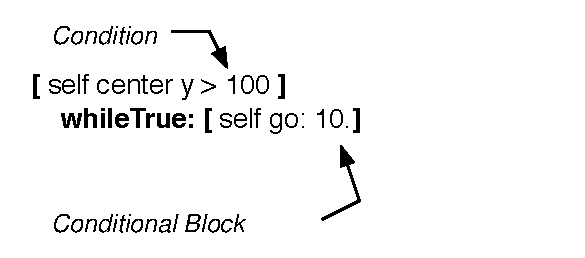
\includegraphics{conditionalLoopsPicture2}
\caption{A \ct{whileTrue:} conditional loop is composed of a condition and a conditional block. The conditional block is only executed when the condition is true. \label{fig:conditionalLoopsPicturehere2}}
\end{center}
\end{figure}

\largecadre{A conditional loop is composed of a condition and a conditional block (that is a sequence of expressions). }


The meaning of the loop is defined by its method name: \ct{whileTrue:} executes its condition and  executes the conditional block when the condition is true.  \ct{whileFalse:} does the same but executes the conditional block only when the condition is false. 

\begin{figure}[h]
\begin{center}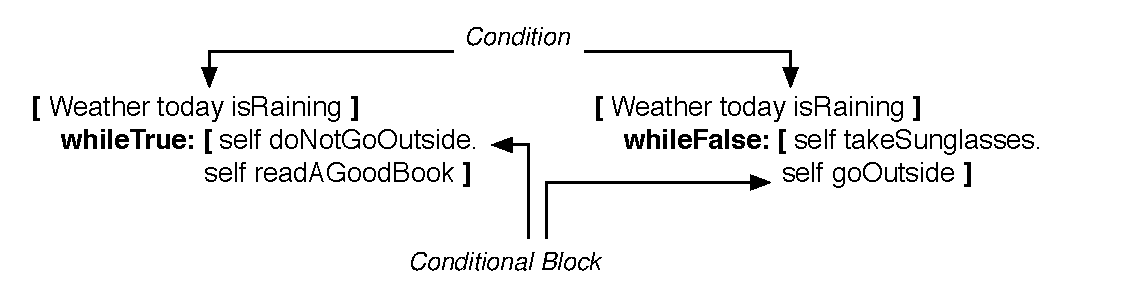
\includegraphics{conditionalLoopsPicture}
\caption{The \ct{whileTrue:} and \ct{whileFalse:} conditional loops are composed of a condition and a conditional block. whileFalse's conditional block is executed when whileFalse's condition is false. WhileTrue's conditional block is executed when whileTrue's condition is true. \label{fig:conditionalLoopsPicturehere}}
\end{center}
\end{figure}

\fprod{the following should be in a frame}
\index{whileTrue:}\ct{whileTrue:} and \index{whileFalse:}\ct{whileFalse:} allow you to define conditional loops \ie the conditional block is repeated while the condition holds. \\
\begin{nalltt}
\textbf{[} condition \textbf{] whileFalse:}
  \textbf{[} conditional messages \textbf{]}

\textbf{[} condition \textbf{] whileTrue:}
  \textbf{[} conditional messages \textbf{]}
\end{nalltt}
\fprod{until here}




\section{Experiences with Traces}
I suggest you add traces in the method you just wrote and analyze the resulting trace. Use also the debugger. Do not hesitate to modify its location in the method. The place where you insert the trace generation has also an impact on the resulting trace. 

For example in method~\ref{mth:uptotrace} I introduced a trace inside the conditional message before they get executed. I obtained the trace shown in Figure~\ref{fig:upTo100Trace}.

\begin{method}\label{mth:uptotrace}
\textbf{upTo100}
   "Make forward the receiver until its ordinates is smaller than 100"

   self north.
   [ self center y > 100 ]
      whileTrue: 
         [\bold{Transcript show: '* ' , self center y asString.}
         self go: 10 ].
   self color: Color green
\end{method}

\begin{figure}[h]
\begin{center}\includegraphics[width=9cm]{upTo100Trace}\end{center}
\caption{The trace of the execution of the method \ct{upTo100}. \label{fig:upTo100Trace}}
\end{figure}


As an alternative experience, introduce the  line \ct{Transcript show: '* ' , self center y asString ; cr.} after the expression \ct{self go: 10} as shown by method~\ref{mth:uptotrace3} or even in the condition before the first  line as shown by method~\ref{mth:uptotrace3}.


\begin{method}\label{mth:uptotrace2}
\textbf{upTo100}
   "Make forward the receiver until its ordinates is smaller than 100"

   self north.
   [\bold{Transcript show: 'c ' , self center y asString; cr.}
   self center y > 100 ]
      whileTrue: 
         [\bold{Transcript show: '* ' , self center y asString; cr.}
         self go: 10 ].
   self color: Color green
\end{method}

\begin{method}\label{mth:uptotrace3}
\textbf{upTo100}
   "Make forward the receiver until its ordinates is smaller than 100"

   self north.
   [ self center y > 100 ]
      whileTrue: 
         [ self go: 10
        \bold{Transcript show: '# ' , self center y asString; cr}] 
\end{method}

Compare the traces produced by the different methods. Look in particular at the final values. 

\ct{whileTrue:} can be converted to \ct{whileFalse:} by negating (logically reverting) the condition.  Use whichever method helps you understand  your program better. Try to define the method \ct{upTo100} that uses \ct{whileFalse:} instead of \ct{whileTrue:}. Then define a method that makes move one pixel at a time. Compare the exact position where it stops.



\subsection*{}
Sometimes defining correct conditional loops is difficult. It is easy to forget to check the condition carefully, and the loop can repeat endlessly. While writing a conditional loop you should always keep in mind that the loop should somehow tend toward the end of the loop \ie\ tend toward a situation that makes the condition not hold anymore. 

Try this experiment: move the robot by using the black halo close to the top edge of the window, \ie\ be sure its y coordinate is smaller than 100. Then invoke the method \ct{upTo100}.  As you see, nothing happens. This as expected: the method is invoked and the expression \ct{self center y > 100} is false, because the position of the robot is smaller than 100. Therefore the conditional block is not executed. 


\section{Stopping an Infinite Loop}
It is not exceptional to write an endless loop. Practically, this happens because the condition expression never returns true for \ct{whileFalse:}; and for \ct{whileTrue:}  it is because the condition never returns false. 

If you do write an endless loop, you can stop \index{stopping an endless loop} it by pressing Apple-. on Mac or Alt . or Control-C on other platforms. Then to understand why the loop did not terminate you can use the debugger that pops up by clicking its Debug button. You can also print some information on the transcript and analyze it.

A conditional loop can endlessly loops when the conditional block does not perform an action that will eventually breaks the condition \ie stop the condition from holding anymore. 

Let's consider this difficult point in the case of our example.  The distance between the robot and the vertical line having 100 as y value gets smaller and smaller. In the example, to be sure that the loop gets a chance to terminate,  the conditional messages should somehow reduce this distance. As long as the robot center's y coordinate is too big (\ct{>= 100}), the loop will continue. So to be sure that the loop will terminate, the conditional block must somehow reduce the robot's y coordinate.  The expression \ct{self go: 10} in the conditional block does this, because the y coordinate gets smaller as the robot moves north.

\begin{figure}[h]
\begin{center}\includegraphics[width=6cm]{PointingSouth}\end{center}
\caption{The situation for the execution of the method \ct{upTo100Infinite}. \label{fig:PointingSouth}}
\end{figure}

Let's look at the case shown in method \ct{upTo100Infinite} (\ref{mth:uptoinfinite}). Here the condition is to stop the loop when the y position of the robot is smaller than 100, that is if the robot arrives above the horizontal line at 100 pixels from the top of the screen.
However as the robot is going to the south as shown in Figure~\ref{fig:PointingSouth}, there is no way that its y coordinate may go below 100. The method~\ref{mth:uptoinfinite} cannot terminate because  the conditional block cannot change the condition to be false. Here, the conditional block increases the value of the y coordinate, therefore the chance that the condition may evaluate to false reduces each repetition. This example is exaggerated but it illustrates clearly the problem of specifying loops that terminate. 

\begin{method}\label{mth:uptoinfinite}
\textbf{upTo100Infinite}
   "Make forward the receiver until its ordinates is smaller than 100"

   \textbf{self south.}
   \textbf{[ self center y > 100 ]}
      whileTrue: \textbf{[ self go: 10 ].}
   self color: Color green
\end{method}

\largecadre{When you are defining a loop always ask yourself if there is a possibility that the condition might never be met. This seems obvious but if the condition does not have a chance to fail the loop will never finish.}

\section{Deeper into \ct{whileTrue:} and \ct{whileFalse:}}
The condition of a conditional loop does not have to contain just a single expression. It can contain a sequence of expressions as long as the last message of the condition returns either true or false. This allows one to express more complicated conditional loops. 


\begin{template}
\textbf{[} self doThis.
anObject doThat.
\emph{self isStillWorking} \textbf{] whileTrue: 
   [}self grumbleAndKeepOnWorking \textbf{]}
\end{template}

Therefore you could change the method \ct{upTo100} to be as method~\ref{mth:notTheSame}. While this method looks nearly the same as \ct{upTo100}, it has sometimes a  different effect. Try to understand what the difference is. For example, add a trace or invoke the debugger in \tmthref{mth:notTheSame} and analyze it. 

\begin{method}\label{mth:notTheSame}
\textbf{notTheSameUpTo100}
   "Move the receiver north until its y coordinate is smaller than 100"

   self north.
   [ self go: 10.
   self center y > 100 ]
      whileTrue: [ ].
   self color: Color green
\end{method}

As the condition is always executed at least once, the main difference is that the robot will move even if it already has a y coordinate smaller than 100.  




\section{A Simple Application}

Conditional loops can be used to ask some values to the user until he gives a correct value. Imagine that you want to ask a user for the number of steps that you should draw. A solution without using a conditional loop is shown in method~\ref{scr:interactiveplus}. First you prompt the user to get a string that represents the number of steps. Then you check whether the data that the user entered represents a number with the \ct{isAllDigits}. When this is the case with convert the string into a number using the method \ct{asNumber} and you perform the loop.


\begin{scriptwithtitle}{Interactive stair}\label{scr:interactiveplus}
| \caro  | 
answer := (FillInTheBlank 
                         request: 'Number of steps' 
                         initialAnswer: '10'). 
answer isAllDigits
   ifTrue: [ \caro := \Turtle new.
           answer asNumber timesRepeat:  
                  [ \caro 
                     go: 10 ; 
                     north ; 
                     go: 10 ;
                     east ]
\end{scriptwithtitle}

Now you can force the user to enter a value that is a number by using a conditional loop that is repeatedly asking for a value if the previous value was not a number.  Script \ref{scr:interactiveplusplus} shows such a version. 

\begin{scriptwithtitle}{Interactive stair}\label{scr:interactiveplusplus}
| \caro answer |
[ answer := (FillInTheBlank 
                         request: 'Number of steps' 
                         initialAnswer: '10'). 
answer isAllDigits] whileFalse: [ ]. 
\caro := \Turtle new.
answer asNumber timesRepeat:  
   [ \caro 
      go: 10 ; 
      north ; 
      go: 10 ;
      east ]
\end{scriptwithtitle}


\section{When to Use \ct{[ ]}}\label{sec:useOfparent}
Now that I presented conditions which require the use of square brackets \ct{[ ]} at different places, you may have difficulties remembering  when to put squared brackets \ct{[ ]}.  There are basically two rules in Smalltalk. You surround an expression or a sequence of expressions with \ct{[} and \ct{]} when:  

\begin{itemize}
\item You need to execute several times the same expression. For example, 
\begin{itemize}
\item \ct{4 timesRepeat: [ \caro go: 10; turnLeft:90 ]} repeats 4 times the messages \ct{\caro go: 10; turnLeft:90}, 
%\item \ct{1 to: 10 do: [:i | Transcript show: i printString ; cr]} repeats ten times the 
%\ct{[:i | Transcript show: i printString ; cr]} which prints the number to the transcript. 
\end{itemize}

\item The expression is executed a variable number of times. For example,

\begin{itemize} 
\item \ct{distance < 200 ifTrue: [ self color: Color red ]} only executes \ct{self color: Color red} under certain circumstances, 
\item \ct{[ self center y > 100 ] whileTrue: [ self go: 10 ]} repeats multiple times conditionally both \ct{self center y > 100} and \ct{self go: 10}, therefore the receiver and the argument are blocks.
\end{itemize}
\end{itemize}

Note that this is an approximation since if you write \ct{1 timesRepeat: [ self go: 120 ]} you still need to put bracket around the expression \ct{self go: 120}. But this is a nice trick to remember. The real definition is: the argument of a conditional message (\ct{ifTrue:}, \ct{ifFalse:}, \ct{ifTrue:ifFalse:}) or conditional loop message (\ct{whileTrue:}, \ct{whileFalse:}) is enclosed in square brackets. The receiver of a conditional loop message (\ct{whileTrue:}, \ct{whileFalse:}) is enclosed in square brackets.

\section{Summary}

\begin{itemize}
\item A conditional loop is composed of a condition and a conditional block that is a sequence of expressions.

\item \index{whileTrue:}\ct{whileTrue:} and \index{whileFalse:}\ct{whileFalse:} allow you to define conditional loops \ie the conditional block is repeated while the condition holds. 

\item When you are defining a loop always ask yourself if there is a possibility that the condition might never be met. This seems obvious but if the condition does not have a chance to fail the loop will never finish.

\item Surround an expression with \ct{[ ]} when (1) you need to execute several times the same expression (\ct{4 timesRepeat: [ self go: 10  ]}) or (2) the expression is not always executed (\ct{dist < 200 ifTrue: [ self color: Color blue ]}).

\end{itemize}


\begin{table}[h]
\small
\centering
\begin{tabular}{||p{5cm}|p{10cm}||} \hline
Method&Description\\ \hline
\begin{nalltt}
\textbf{[} aCondition \textbf{] whileFalse:}
  \textbf{[} SequenceOfMessages \textbf{]}
\end{nalltt}
&Execute \ct{aCondition};  if it is false execute \ct{SequenceOfMessages} and repeat this step.  If \ct{aCondition} is true, pass to the next expression without executing  \ct{SequenceOfMessages}. \\  \hline

\begin{nalltt}
\textbf{[} aCondition \textbf{] whileTrue:}
  \textbf{[} SequenceOfMessages \textbf{]}
\end{nalltt} 
&Execute \ct{aCondition};   if it is true execute \ct{SequenceOfMessages} and repeat this step.  If \ct{aCondition} is false, pass to the next expression without executing  \ct{SequenceOfMessages}. \\  \hline \hline
\end{tabular}
\end{table}




\ifx\wholebook\relax\else\end{document}\fi





